\documentclass[12pt]{article}


\usepackage{graphicx}
\graphicspath{ {./Figures/} }
\usepackage{amsmath}
\usepackage{hyperref}

\title{Social Mixing Matrix Literature Review and an Intuitive Approach for the $\mathcal{R}_{0}$}

\author{GitHub: \url{https://github.com/epidemic-research-team/}}

\begin{document}
\maketitle

\section{Introduction}

Standard epidemic models, such as SIR, SIS and their extensions  SIRS, MSEIRS, SEIR are well established mathematical methods that simulate the spread of an infectious decease \cite{keeling2008modeling, ma2009mathematical, li2018introduction}. One limitation of these models is that they base their prediction on the a-priori assumption that the rate of contact in a population is constant across environments and age groups. As a result, these methods neglect the vital component of how populations interact. Therefore, researchers who solely rely on the SIR/SIS family of models often formulate contact rates ($\sigma$) and reproduction numbers ($\mathcal{R}_{0} $) based on assumptions and non-data driven hypotheses. As a reminder, $\mathcal{R}_{0} $ is the "\textit{basic reproduction number $\mathcal{R}_{0}$, which is defined as the average number of secondary infections produced when one infected individual is introduced into a host population where everyone is susceptible}" \cite[p.21]{ma2009mathematical}. In general, $\mathcal{R}_{0} >\sigma$ but in many models $\mathcal{R}_{0} =\sigma$. 

Social Mixing Matrices (SMMs) are considered important tools for formulating realistic $\mathcal{R}_{0}$ and $\sigma$. SMMs capture social distancing patterns based on direct observations and surveys and as a result they provide crucial information to both scientists and public officials on how a directly transmitted infectious decease is spreading. Because of the granularity of the data that SMMs offer, their use has the potential to increase model robustness and prediction accuracy compared to models that rely solely on indirect data \cite{Mossong:2008, Baguelin:2013}. 

\section{Literature Review}

On their study, \cite{Diekmann:2010} explored the construction of the called next generation matrices (NGMs). NGMs are a vital part of the SMMs construction and utilisation process. Many papers that have used SMMs, one way or the other, they had to transform their initial population interaction matrix to be NGM compliant in order to adequately compute the integral $\mathcal{R}_{0} $ and $\sigma$ \cite{Mossong:2008, Fumanelli:2012, Klepac2020}. In other words, NGMs show the number of novel infections from each category (age groups, gender groups, etc) in consecutive generations \cite[p.874]{Diekmann:2010}. From the NGM, we can map the $\mathcal{R}_{0}$ to the dominant eigenvalue of the matrix. The ODE models that are used in epidemiology are linearised and form a Jacobian matrix \cite[Section 2.1.2]{keeling2008modeling}, then \cite{Diekmann:2010} showed how to decompose this matrix into a transition component $\Sigma$ (change in state) and a transmission part $T$ (new infections). 

A landmark SMM based study was POLYMOD \cite{Mossong:2008} that includes $n=7,290$ participants from 8 European countries between years 2005-2006. This is the first study of such inter-state scale and since then it has been widely used amongst publications in the field. POLYMOD, contains information for $97,904$ contacts grouped by age, gender, type of contact (physical, conversational), place and frequency. The study expanded the pool of potential information that researchers for epidemiological deceases could access. In their results, the authors showed some interesting cultural outcomes. For example, using countries as dummy variables do seem to make a difference in the social mixing matrix. For instance, German participants showed per daily average $\mu=8$ fewer number of contacts compared to their Italian counterparts $\mu=20$. 

One limitation with the POLYMOD study is the population bias that exhibits on children and young adult ages as the focus of the study has been set deliberately on these age groups. The reason is that the infectious decease that the authors studied (influenza) were most likely to be transmitted through young ages. For example, 38\% of the participants are under 20 years old of age and 12\% were over 60 years old. At the time of survey, the European average for these 8 countries for 20 y and under was 17\% and the same average for 60 y and over was 21\%. As a reference, the EU average for 20 y and under was 16\% and 23\% respectively. There is also a small change over the years, in 2018 (the same year as the BBC Pandemic survey in UK) the population in the 8 countries for 20 y and under was 15\% and for 60y and over was 25\%. The inclusion of developing Eastern European countries has not managed to reverse the ageing population that developed countries suffer from. The subsequent rapid development of the new European Union countries has affected them with the same problem of an ageing population \footnote{Information sourced from Eurostat data [demo\_pjanbroad]}. Another potential issue with the POLYMOD data is the time that has passed since the study was contacted. Since then, social behaviours and patterns might have changed dramatically. 

Considering the aforementioned limitations that the POLYMOD data suffer from, \cite{Klepac2020}, with the assistance of BBC Pandemic project, conducted a large scale population and social behaviour survey in UK, 2017-2018. The study included $n=38,000$ volunteers between 13-90+ by contact type (physical, conversational) and by social environment (work, home, etc) . The survey, groups the individuals in 5 year age segments, up to 75+ for whom there is a single category. To construct the social mixing matrix \cite{Klepac2020} start from the \textit{raw contact matrix} ($M$), where its elements are $m_{ij}=\frac{t_{ij}}{n_{j}}$. For $t_{ij}$ is the total number of contacts, within 24h, between the reference age group $j$ and people in age group $i$. Then, we compute the average number of contacts per surveyed person $j$ by $m_{ij}=\frac{t_{ij}}{n_{j}}$. Next, the authors create a reciprocal matrix, or \textit{population contact matrix} $C$, which is a biased version of the matrix $M$. The matrix $C$, uses ONS population data for 2018 $w$, for each age group, as a "prior" element that adds to the $m_{ij}$ in order to get more realistic results, $c_{ij}=\frac{1}{2}(m_{ij} + m_{ij}\frac{w_{i}}{w_{j}})$. 

The BBC Pandemic survey from \cite{Klepac2020} covers most of the limitations that POLYMOD study \cite{Diekmann:2010} has but BBC Pandemic has its own drawbacks too. For instance, because the BBC app allowed users from 13 y and more the survey does not contain information for ages below 13 y. For the study of infectious deceases that are transmitted more easily amongst children there is a gap in the survey. There is also an element of population bias considering the fact that the sample has not been selected randomly from the overall geographical population. It might be that population from big cities dominate the study. Also, the survey is not gender specific, whereas POLYMOD is. 

A study on the magnitude of \cite{Klepac2020} is comprehensive and extensive but also costly, time consuming and logistically complicated. As alternative, researchers used statistical methods to map the social mixing characteristics from the 8 countries of \cite{Diekmann:2010} into other geographic areas and from there to infer results. These methods, could potentially by utilised in order to expand research on local authority level in UK or to other countries. For instance, \cite{Fumanelli:2012} used census data from 28 European countries (household, work, education etc) in order to construct synthetic NGM. In general, they assume a uniform distribution to depict the contacts amongst individuals and then use empirical evidence from past research as a prior to modify these contact rates according to the social setting (work, household, school, etc) before they construct the average frequency of contacts matrix $M$ that leads to the NGM matrix.

Other papers that have evaluated and expanded the POLYMOD survey using statistical methods include \cite{Kiesha:2017}, where the authors sourced socio-demographic data from 152 countries in order to project the POLYMOD from 8 to 144 countries, using a hierarchical Bayesian model and MCMC to sample the posterior parameters.

\section{Computation of $\mathcal{R}_{0}$ from NGM}
\label{sec:2}

Before we delve into the work of \cite{Diekmann:2010} and how to derive the $\mathcal{R}_{0}$ using the NGM, we should first briefly discuss what is the $\mathcal{R}_{0}$. For readers new to epidemiology, there often is a mistaken notion that $\mathcal{R}_{0}$ is an infection rate, or the rate of spread of a disease. This is incorrect, the $\mathcal{R}_{0}$ is a dimensionless number (scalar) that as we explained in the beginning of the text, it shows the \textbf{average} number of spread amongst the population \cite{ma2009mathematical, Jones:2007}. Overall, as \cite{Jones:2007} explains 

\begin{equation*}
\mathcal{R}_{0}= \bigg(\frac{\mbox{ infection}}{\mbox{ contact}}\bigg) \bigg(\frac{\mbox{ contact}}{\mbox{ time}}\bigg) \bigg(\frac{\mbox{ time}}{\mbox{ infection}}\bigg) 
\end{equation*}

alternatively

\begin{equation}
\mathcal{R}_{0}= \tau \bar{c} d
\label{eq:10}
\end{equation}

with $\tau$ is the probability of transmission during a contact, $\bar{c}$ is the \textbf{average} rate of contact between individuals and $d$ is the duration of the infectiousness \cite[p.1]{Jones:2007}. Mapping these to a simple SIR model

\begin{align*}
\dot{S} & =  - \beta \frac{SI}{N} \\
\dot{I}  & =  \beta \frac{SI}{N} - \gamma I  \\
\dot{R}  & =  \gamma I 
\end{align*}

$\beta=\tau \bar{c}$, the effective contact rate (force of infection) equals the product of probability of transmission with the average rate of contacts between the population groups.  Also, $d=\gamma^{-1}$, the duration of the infectiousness is the inverse removal rate. Therefore, for an epidemic to spread intuitively needs the infection rate to be $I>0$

\begin{align*}
\beta \frac{SI}{N} - \gamma I  & >  0 \\
\beta \frac{SI}{N}  & >  \gamma I  \\
\mathcal{R}_{0} =  \frac{\beta}{\gamma } & >  0 
\end{align*}

Overall, what we are trying to achieve by calculating the $\mathcal{R}_{0} $ is to create a value that summarises the number of newly infected by averaging the number new infections over all possible infected types \cite[p.3]{Jones:2007}. For complex systems (SEIR) a way to compute this number is by utilising matrix algebra. As \cite{Diekmann:2010} to find the average value we can use the spectral radius (dominant eigenvalue) of the NGM, which is similar to the geometric mean. 


\subsection{Next Generation Matrices: SEIR}
\label{sub:2.1}

In their paper, \cite[p.875]{Diekmann:2010} use a SEIR model with 2 exposed categories as an example ($E_{1}, E_{2}$).

\begin{align*}
\dot{S} & =  \mu N - \beta\frac{SI}{N} + \mu S \\
\dot{E}_{1}  & =  \rho \beta \frac{SI}{N} - (\nu_{1} + \mu)\dot{E}_{1} \\
\dot{E}_{2}  & =  (1 - \rho) \beta \frac{SI}{N} - (\nu_{2} + \mu)\dot{E}_{2}\\
\dot{I}  & =  \nu_{1} \dot{E}_{1}  + \\nu_{2} \dot{E}_{2}  - (\gamma + \mu) I \\
\dot{R}  & =  \gamma I - \mu R\\
\end{align*}

where $\mu$ per capita birth and death rates, $\beta$ the transmission rate, $\nu_{i}\in\{1, 2\}$ the rates of leaving the respective latency states $E_{i}$, $\gamma$ the rate of leaving the infection state and $N=S + E_{1} + E_{2} + I + R$.
Let $\dot{x} = (E_{1}, E_{2}, I)^{T}$, and we want to decompose the system to have the form

\begin{equation}
\dot{x} = (T + \Sigma)x
\end{equation} 

where matrix $T$ corresponds to transmissions and matrix $\Sigma$ to transitions. 

According to \cite{Diekmann:2010}, the role of $T$ and $\Sigma$ is similar to the sufficient statistics, as all information that is required is included in the decomposition. For the transmission matrix $T$, we create a matrix with infected states, using indices $i, j\in {1, 2, 3}$ and the record $T_{ij}$ is the rate of infection term; individuals from state $j$ infects individuals in $i$. If the element in $T_{ij}$ is 0, then there is no chance of transmission.  Therefore, 

\begin{equation*}
T=
\begin{pmatrix}
0 & 0 & \rho \beta\\
0 & 0 & c (1-\rho)\beta\\
0 & 0 & 0
\end{pmatrix}
\end{equation*}

and 

\begin{equation*}
\Sigma=
\begin{pmatrix}
-(\nu_{1}+\mu) & 0 & 0\\
0 & -(\nu_{2}+\mu) & 0\\
\nu_{1} &  \nu_{2}& -(\gamma + \mu)
\end{pmatrix}
\end{equation*}

hence we solve for the NGM with large domain ($K_{L}$)

\begin{equation*}
K_{L} = -T\Sigma^{-1} = 
\begin{pmatrix}
0 & 0 & \rho \beta\\
0 & 0 & c (1-\rho)\beta\\
0 & 0 & 0
\end{pmatrix}
\times
\begin{pmatrix}
-(\nu_{1}+\mu) & 0 & 0\\
0 & -(\nu_{2}+\mu) & 0\\
\nu_{1} &  \nu_{2}& -(\gamma + \mu)
\end{pmatrix}
\end{equation*}

the dominant eigenvalue of this matrix $K_{L}$ is the $\mathcal{R}_{0}$

\begin{equation}
\mathcal{R}_{0} = \bigg( \frac{\rho \nu_{1}}{\nu_{1} + \mu} + \frac{(1-\rho) \nu_{2}}{\nu_{2} + \mu}  \bigg) \frac{\beta}{(\gamma + \mu)}
\end{equation}

or similarly, by using the equation of NGM

\begin{equation}
K=E^{T}K_{L}E=-E^{T}T\Sigma^{-1}E
\end{equation}

with $E$ being a matrix that its columns contain unit vectors the non-zero rows of matrix $T$, which leads

\begin{equation}
\mathcal{R}_{0}  = \rho (K) = \frac{1}{2} \bigg( trace(K) + \sqrt{trace(K)^{2} + 4det(K)} \bigg)
\label{eq:8}
\end{equation}

The above case can be expanded for two groupings of individuals (male and female).

\subsection{Next Generation Matrices: BBC Pandemic Survey}
\label{sub:2.2}

The NGM of \cite{Diekmann:2010} can be linked with \cite{Klepac2020} matrix $C$ by 

\begin{equation}
NGM  = \frac{\mathcal{R}_{0}}{\rho(C)} C
\end{equation}

Analogous to the Equation \ref{eq:8}, the $\rho(C)$ is the largest eigenvalue of $C$. As in PCA, the eigenvector associated with $\rho(C)$ shows which age group dominates in the social interactions and explain more the overall data variance. Therefore, following \cite{Diekmann:2010} examples we find the NGM and we already have $\rho(C)$ and $C$ and we extract $\mathcal{R}_{0}$.

\begin{equation}
\mathcal{R}_{0} = NGM \times C \rho(C)^{-1}
\label{eq:9}
\end{equation}

\subsection{Next Generation Matrices: SIR}
\label{sub:2.3}

We saw in sub-Section \ref{sub:2.1} how to use \cite{Diekmann:2010} method to compute the NGM and subsequently the $\mathcal{R}_{0}$. Next, \cite[p.4]{Fumanelli:2012} provided an example of how to link \cite{Diekmann:2010} NGM method to a SIR model. Specifically, let the force of infection be $\lambda_{i}$ of a SIR model to be a linear combination of the average frequency matrix $M_{ij}$, where it shows the frequency of contacts between age groups $i$ and age groups $j$, and a  transmissibility coefficient $\beta_{i}$, which accounts the probability of infenction per contact. The matrix $M_{ij}$ is similar to BBC Pandemic \cite{Klepac2020} matrix $C_{ij}$ ($C$ is a population biased $M$, see sub-Section \ref{sub:2.2}). 

The equations of the SIR model are

\begin{align*}
\dot{S} & =  \mu N - \beta M\frac{SI}{N} - \mu S\\
\dot{I}  & =  \beta M\frac{SI}{N} - (\gamma + \mu) I  \\
\dot{R}  & =  \gamma I - \mu R
\end{align*}

unlike the examples in \cite{Diekmann:2010}, the authors do not use a population constant; nevertheless, we add them for consistency reasons, $\mu$. Then, we calculate the $\mathcal{R}_{0}$ as the spectral radius of the NGM 

\begin{equation}
\mathcal{R}_{0} = \rho(\beta\gamma^{-1}M)
\end{equation}

this is slightly different from \cite{Klepac2020} approach to compute $\mathcal{R}_{0}$ (Equation \ref{eq:9}). 

\subsection{Next Generation Matrices: SIR-COVID}
\label{sub:2.4}

The aim of this research is to employ the work of \cite{Diekmann:2010} and \cite{Fumanelli:2012} in computing the $\mathcal{R}_{0}$ in the epidemiological model from \cite{Gareth:2013}. The model will be adapted to COVID-19 cases and to include social mixing matrix data instead of the sexual contact matrix that the authors used. The compartmental transmission model has a form as shown in Figure \ref{fig:model} \cite[p.5]{Gareth:2013}. From the Figure \ref{fig:model}, the surveyed population is divided into the following non-overlapping compartments: $S$ is for individuals who are at risk of Covid-19 infection, $I$ is for infected individuals, $G$ is for infected who developed serious symptoms and required ICU admission, $P$ is those who have recovered, and are seropositive and immune, $N$ is for individuals who are recovered, immune but seronegative. The indices $g$, $a$ and $s$ indicate that every compartment is stratified by gender, age and level of social activity. Movements between compartments are occurring at per capita rates specified by the following parameters: $\lambda$ is the \textbf{force of infection} dependent on the proportion of individuals in $I$, \textbf{PSC} is the probability of becoming seropositive, \textbf{WIP} is the Covid-19 incubation period, \textbf{DAI} is the duration of asymptomatic (i.e. without Covid-19) infection symptoms, \textbf{DWT} is the duration of treatment for Covid-19, and \textbf{DI} is the duration of immunity. Subscripts denote stratification of parameters: for example, \textbf{DWT}$_{g}$ means that in our model this parameter is gender-dependent.

\begin{figure}[h!]
\centering
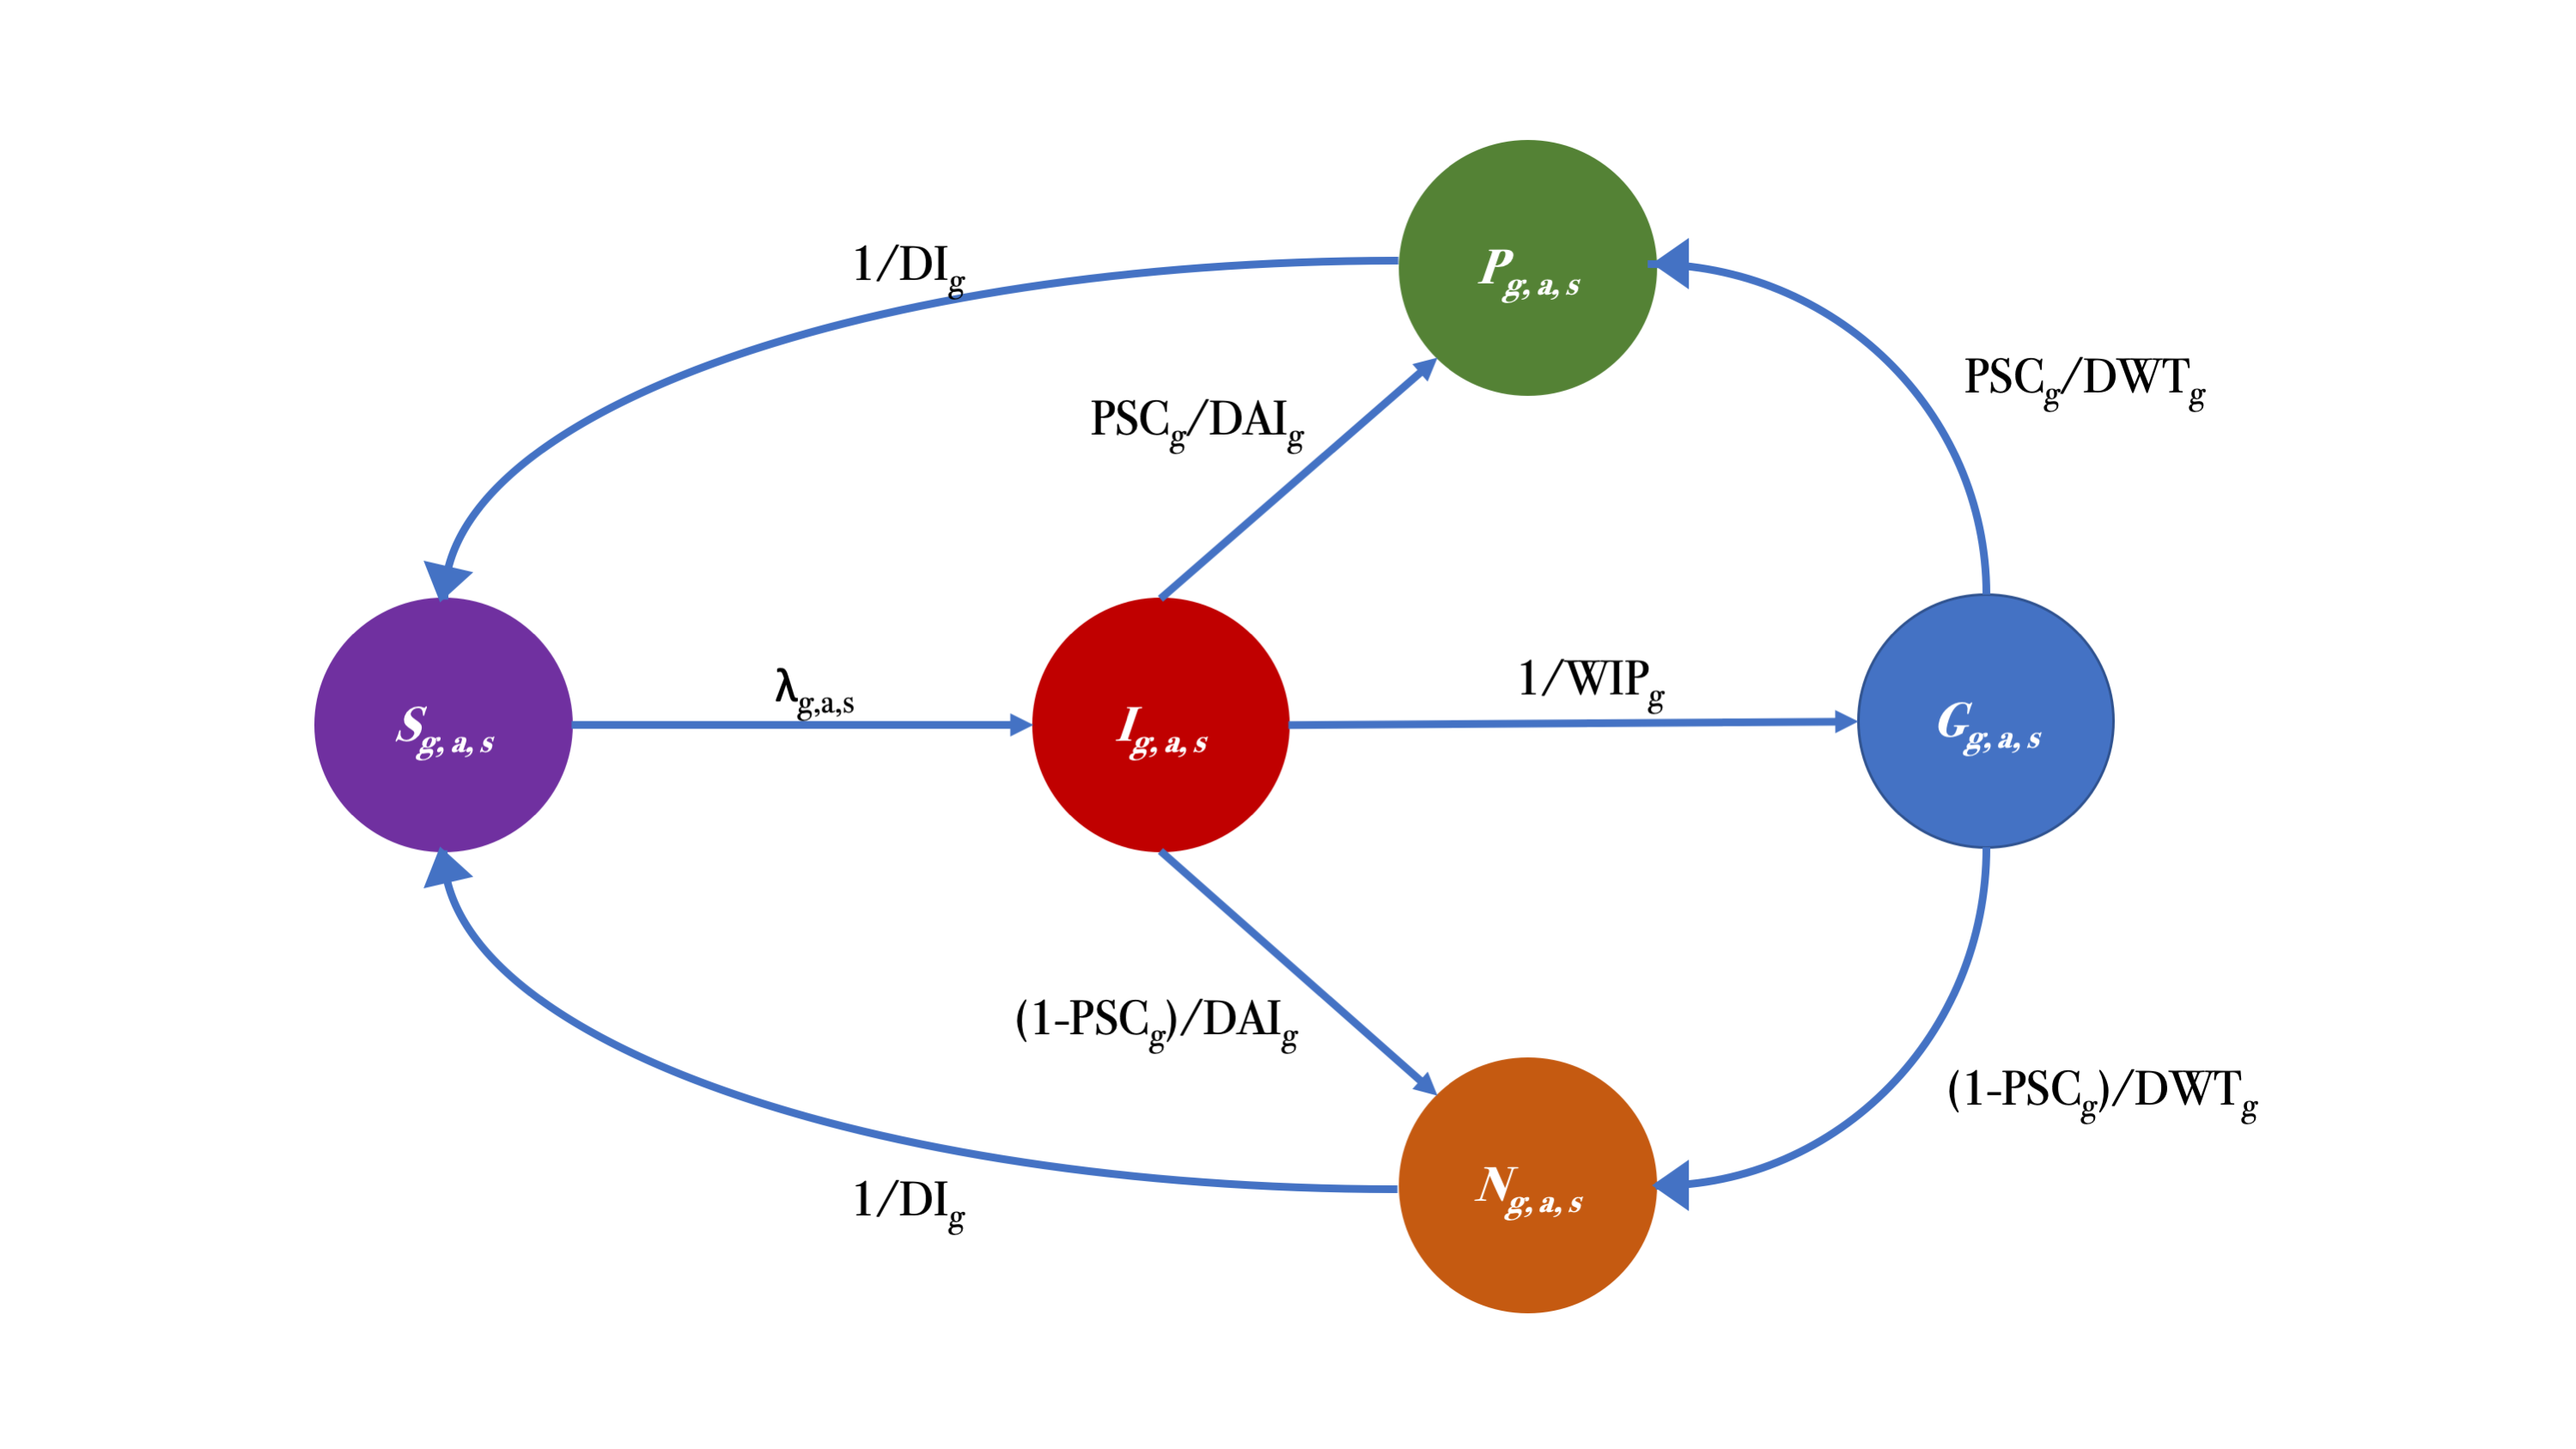
\includegraphics[width=1\textwidth]{COVIDb}
\caption{A compartmental Covid-19 transmission model.}
\label{fig:model}
\end{figure}

The system of ODEs is then formulated as follow

\begin{align*}
\dot{S}_{g,s,a} & =  -\lambda_{g,s,a}(t)S_{g,s,a} + (P_{g,s,a} + N_{g,s,a})/DI_g + \frac{1}{r}S_{g,s,a-1} - \frac{1}{r}S_{g,s,a} + \\
& \quad \frac{1}{R}\sum_{g,s}(S_{g,s,20} + I_{g,s,20} + G_{g,s,20} + P_{g,s,20} + N_{g,s,20}) \times \\
& \quad \delta_1(a)(\pi_1\delta_1(s) + \pi_2\delta_2(s) + \pi_3\delta_3(s) + \pi_4\delta_4(s)) \\ 
\dot{I}_{g,s,a}  & =  \lambda_{g,s,a}(t)S_{g,s,a} - (1/WIP_g + 1/DAI_g)I_{g,s,a} + \frac{1}{r}I_{g,s,a-1}-\frac{1}{r}I_{g,s,a} \\
\dot{G}_{g,s,a}  & =  I_{g,s,a}/WIP_g - G_{g,s,a}/DWT_g + \frac{1}{r}G_{g,s,a-1} - \frac{1}{r}G_{g,s,a} \\ 
\dot{P}_{g,s,a}  & =  PSC_g(I_{g,s,a}/DAI_g + G_{g,s,a}/DWT_g) - P_{g,s,a}/DI_g + \frac{1}{r}P_{g,s,a-1} - \frac{1}{r}P_{g,s,a} \\
\dot{N}_{g,s,a}  & =  (1-PSC_g)(I_{g,s,a}/DAI_g + G_{g,s,a}/DWT_g) - N_{g,s,a}/DI_g + \frac{1}{r}N_{g,s,a-1}-\frac{1}{r}N_{g,s,a} \\
\end{align*}

the stochastic compartmental system has in total 5 states, $T_{total \quad population} = S + I + P + N + G$; of which two are infected states $I$ and $G$ and three uninfected states $S$, $P$ and $N$. The total population remains constant by adding an ageing term in the susceptible compartment, $\frac{1}{R}\sum(\dots)\times\delta\pi$ \cite[p.7]{Gareth:2013}. The ODE $I$ is the state that contains the rate of infection term $\lambda$. The model is high dimensional since it involves the non-linear ODEs parameters that need to be calibrated ($\lambda, WIP, DAI, DWT, DI$). At the infection free state, the number of susceptible equals the total population $S=T{total \quad population}$. 

Following \cite{Fumanelli:2012, Baguelin:2013, Klepac2020}, we will expand \cite{Gareth:2013} by including in our research a social mixing matrix (POLYMOD or BBC Pandemic) to infer the $mathcal{R}_{0}$ and also we will consider the level of intervation and the impact it has on the social mixing patterns \cite{Kiesha:2017}. The current paper from \cite{Gareth:2013} is using a sexual transmission matrix with dimensions ($2 \times 4 \times 4 \times 9 \times 9$) for $g=1|males$ and $g=2|females$, four sexual activity groups $(s\in {1, \dots ,4})$ and a 9-bracket age group. In this initial stage of the model we will simplify the social distancing matrix by using only the age group as dimensions, we will move into more complex applications later.

The first step is to construct the NGM matrix \cite{Diekmann:2010} by using the survey data. In this example we will construct the NGM based on the BBC Pandemic data but following \cite{Fumanelli:2012} approach for the SIR model. 



From \cite{Klepac2020}, we compute the contact matrix $M$ as a linear combination of age-specific contacts by context (home $h$, work $w$, school $s$, other $r$) and type (conversational $Co$ or physical $Ph$) using the \textit{population contact matrices} $C$. We also adjust the population contact matrices by a factor, based on temporal data collected from Google AI and Apple mobility reports \footnote{All data, including COVID, social distancing matrices, mobility reports, ONS and census UK specific data can be accessed in GitHub  \url{https://bit.ly/2KNP06w}}.

\begin{equation}
M = H_{mob}C^{h} + W_{mob}C^{w} + S_{mob}C^{s} + R_{mob}C^{r}
\end{equation}

where $H_{mob}, W_{mob}, S_{mob}, R_{mob}$ are the mobility factors of home, work, school and other. The mobility factor matrices can be temporal, as a function of time similar to the ODEs or fixed. For the latter, we can use an average value of mobility reduction from the mobility reports. It is recommended though, because population movement restrictions could play a very significant role for the spread or not of the decease to utilise a temporal format. For instance, the mobility factor of $H$ will have the approximate form:

\begin{equation*}
H=
\begin{pmatrix}
0.3 & 0 & \dots & 0\\
0 & 0.3 &  & 0\\
\vdots &  &  & \vdots  \\
0 &  0 & \dots & 0.3
\end{pmatrix}
\end{equation*}

From \cite[p.9]{Gareth:2013}, we know the force of infection (effective contact rate) is

\begin{equation}
\lambda_{g,s,a}=\beta_{g}\sum_{s^{'}, \alpha^{'}} \bigg\{ c^{*}_{g,s,s^{'},\alpha,\alpha^{'}} \rho^{*}_{g,s,s^{'},\alpha,\alpha^{'}} \frac{I_{g^{'}, s^{'}, \alpha{'}}}{S_{g^{'}, s^{'}, \alpha{'}} + I_{g^{'}, s^{'}, \alpha{'}} + G_{g^{'}, s^{'}, \alpha{'}} + P_{g^{'}, s^{'}, \alpha{'}} + N_{g^{'}, s^{'}, \alpha{'}} } \bigg\}
\label{eq:11}
\end{equation}

From Equation \ref{eq:11}, we drop the $\rho^{*}_{g,s,s^{'},\alpha,\alpha^{'}}$ conditional probability of contact between sexual partners. Instead, we assume a uniform distribution amongst age groups to contact and transmit the disease. We can add this parameter on a later stage if needed and we think that specific age groups $j$ have more probability of transmitting the decease when contacting age groups $i$. In the next formula we replace the contact rate $c$ with the social mixing matrix that we constructed $M$

\begin{equation}
\lambda_{a}=\beta_{g}\sum_{s^{'}, \alpha^{'}} \bigg\{ M_{a} \frac{I_{g^{'}, s^{'}, \alpha{'}}}{S_{g^{'}, s^{'}, \alpha{'}} + I_{g^{'}, s^{'}, \alpha{'}} + G_{g^{'}, s^{'}, \alpha{'}} + P_{g^{'}, s^{'}, \alpha{'}} + N_{g^{'}, s^{'}, \alpha{'}} } \bigg\}
\label{eq:11}
\end{equation}

\subsection{Incorporate Local Authority Districts Information to COVID Model}
\label{sub:2.5}

As a final step for the expansion of \cite{Gareth:2013} paper is to utilise the statistical information we have in Local Authority Districts (LAD) level or in NUTS3 level. 

TBD

Brief: Use $\beta$ from \cite{Gareth:2013} as a weight for local authority - how probable is to get infected there. Use Google mobility time-series for local authority. Create a matrix $(t \times 150 \times 19 \times 19)$ and apply it to $\lambda$ from \cite{Gareth:2013}.

\bibliographystyle{abbrv}
\bibliography{simple}

\end{document}
This is never printed
